\chapter{ROBOTSKI SUSTAV I SIMULACIJSKO OKRUŽENJE}
\label{ch:sustav}

Ovo poglavlje opisuje robotski sustav na kojem su razvijena i ispitana oba pristupa
upravljanju, modele vrata koji čine radnu okolinu, postupak izrade simulacijskog modela te
programsku arhitekturu koja povezuje simulator i upravljački kod. Cijeli je rad proveden u
simulaciji; razlozi i posljedice tog izbora navedeni su u potpoglavlju \ref{sec:isaac}.

\section{KMR iiwa — mobilna platforma i manipulator}
\label{sec:kmr}

KUKA KMR iiwa (slika \ref{fig:kmr-iiwa}) mobilni je manipulator sastavljen od dviju serijskih komponenti: omnidirekcijske
mobilne platforme KMP 200 omniMove i laganog robota LBR iiwa. Na prirubnicu manipulatora
dodana je prihvatnica opisana u potpoglavlju \ref{sec:gripper}. Kombinacija pokretljive
platforme i osjetljivog manipulatora namijenjena je radu bez zaštitne ograde, u okolini u
kojoj se robot kreće između radnih mjesta \cite{kuka2024kmriiwa}.

\begin{figure}[H]
    \centering
    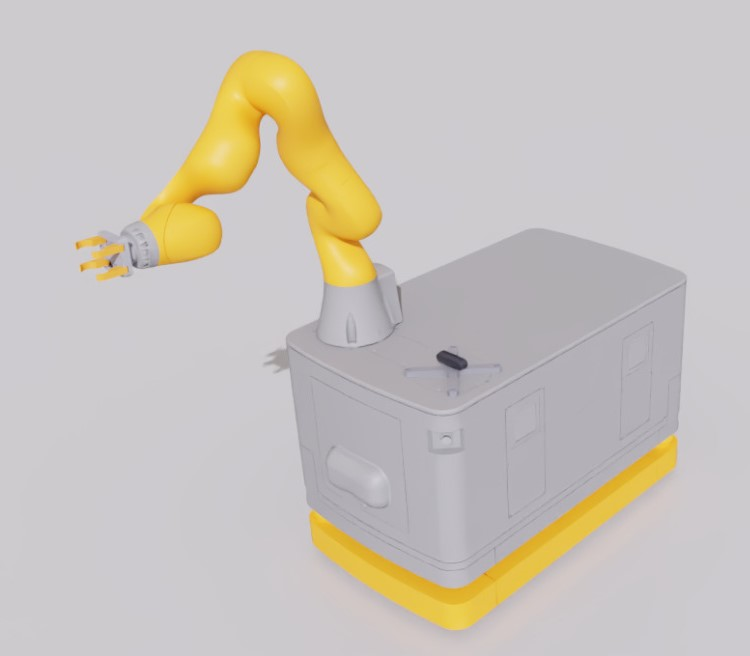
\includegraphics[width=0.7\textwidth]{figures/kmr_iiwa_isaac.jpg}
    \caption{Mobilni manipulator KMR iiwa u simulacijskom okruženju}
    \label{fig:kmr-iiwa}
\end{figure}

\subsection{Mobilna platforma}
\label{sec:platforma}

Platforma se giba pomoću četiriju Mecanum kotača (slika \ref{fig:mecanum-wheel}). Svaki se kotač sastoji od niza valjaka
postavljenih pod kutom od 45\textdegree{}{} u odnosu na os kotača, čime se postiže
omnidirekcijsko gibanje --- platforma se može gibati u proizvoljnom smjeru u ravnini i
istovremeno se zakretati, bez potrebe za promjenom orijentacije prije translacije. Ta je
osobina bitna za zadatak otvaranja vrata, jer omogućuje da baza slijedi luk krila bez
manevriranja. Tehnički podaci mobilne platforme nalaze se u tablici \ref{tab:platforma}.

\begin{figure}[H]
    \centering
    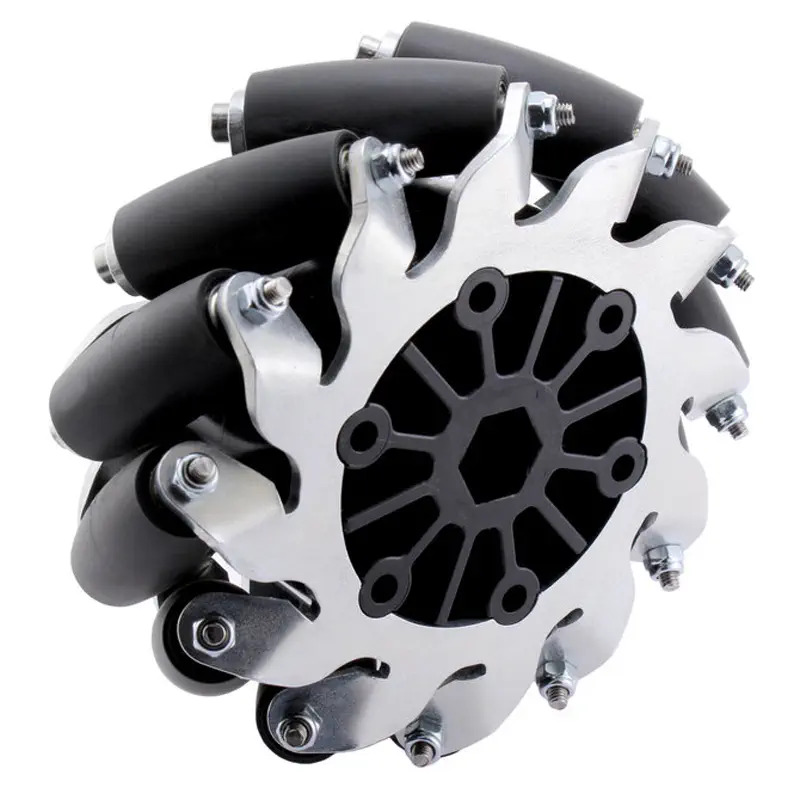
\includegraphics[width=0.45\textwidth]{figures/mecanum.jpg}
    \caption[Građa Mecanum kotača]{Građa Mecanum kotača \cite{mecanumsource}}
    \label{fig:mecanum-wheel}
\end{figure}

\begin{table}[H]
    \centering
    \caption{Tehnički podaci mobilne platforme}
    \label{tab:platforma}
    \begin{tabular}{@{}ll@{}}
        \toprule
        Veličina                                & Vrijednost                            \\
        \midrule
        Dimenzije (V\,$\times$\,Š\,$\times$\,D) & 700\,$\times$\,1080\,$\times$\,630 mm \\
        Masa                                    & 390 kg                                \\
        Najveća nosivost                        & 170 kg (200 kg bez manipulatora)      \\
        Brzina u uzdužnom smjeru                & najviše 3.6 km/h                      \\
        Brzina u poprečnom smjeru               & najviše 2.0 km/h                      \\
        Promjer kotača                          & 250 mm                                \\
        Klasa čistoće                           & ISO 5                                 \\
        \bottomrule
    \end{tabular}
\end{table}

\subsection{Manipulator LBR iiwa 7 R800}
\label{sec:lbr}

Korišten je manipulator LBR iiwa 7 R800, redundantna kinematička struktura sa sedam
rotacijskih osi. Za ovaj je rad ključno da manipulator ima senzor momenta u svakoj osi, što
omogućuje procjenu sile i momenta na vrhu alata bez zasebnog senzora sile na zapešću.
Postupak te procjene opisan je u poglavlju \ref{ch:procjena}. Sedma os čini strukturu
redundantnom u odnosu na šest stupnjeva slobode zadatka, pa isti položaj i orijentaciju vrha
alata ostvaruje kontinuum konfiguracija --- svojstvo koje se u poglavlju \ref{ch:rezultati}
pokazalo dosta važnim. Tehnički podaci manipulatora nalaze se u tablici \ref{tab:lbr}.

\begin{table}[H]
    \centering
    \caption{Tehnički podaci manipulatora LBR iiwa 7 R800}
    \label{tab:lbr}
    \begin{tabular}{@{}ll@{}}
        \toprule
        Veličina                    & Vrijednost         \\
        \midrule
        Nazivna nosivost            & 7 kg               \\
        Broj osi                    & 7                  \\
        Doseg                       & 800 mm             \\
        Izvedba zapešća             & u liniji           \\
        Prirubnica na osi 7         & DIN ISO 9409-1-A50 \\
        Ponovljivost pozicioniranja & $\pm$0.1 mm        \\
        Točnost momenta po osi      & $\pm$2 \%          \\
        Masa                        & 23.9 kg            \\
        Stupanj zaštite             & IP54               \\
        Položaj ugradnje            & pod, strop, zid    \\
        \bottomrule
    \end{tabular}
\end{table}

Granični momenti pojedinih zglobova navedeni su u tablici \ref{tab:momenti}.

\begin{table}[H]
    \centering
    \caption{Granični momenti zglobova manipulatora}
    \label{tab:momenti}
    \begin{tabular}{@{}lccccccc@{}}
        \toprule
        Zglob               & 1   & 2   & 3   & 4   & 5   & 6  & 7  \\
        \midrule
        Granični moment, Nm & 176 & 176 & 110 & 110 & 110 & 40 & 40 \\
        \bottomrule
    \end{tabular}
\end{table}

\section{Prihvatnica}
\label{sec:gripper}

Za hvatanje kvake izrađena je prilagođena prihvatnica (slika \ref{fig:gripper-render}). Budući da se rad provodi isključivo u
simulaciji, a stvarni prihvatni uređaj nije bio zadan, prihvatnica je oblikovana kao
zamjenjiva komponenta, tj. upravljanje njome potpuno je odvojeno od ostatka softvera
(potpoglavlje \ref{sec:ros2}), pa se može zamijeniti bez izmjena u ostatku sustava.

Prihvatnica ima četiri prsta raspoređena u dva para koja se zatvaraju duž osi $x$ baze, dok
uhvaćena šipka leži duž osi $y$. Svaki prst na sebi ima utor čiji je unutarnji luk prilagođen
šipki kvake promjera 28 mm. Pri potpuno zatvorenom hvatu otvor između prstiju uži je od šipke,
pa hvat ne počiva na geometrijskom dosjedanju nego na sili pogona i popustljivosti prstiju.
Time se izbjegava zazor koji bi pri vučenju vrata dopustio da se kvaka pomiče unutar hvata.
Položaj vrha alata (\textit{TCP}, engl. \textit{tool center point}) može se vidjeti na slici \ref{fig:gripper-tcp}.
Značajke prihvatnice nalaze se u tablici \ref{tab:gripper}.

Parovi prstiju ne gibaju se savršeno simetrično, pa se predmet ne centrira sam od sebe.
Ta se asimetrija ne pokušava ukloniti, nego se mjeri: tijekom prilaza kvaki uspoređuju se
položaji suprotnih prstiju i iz razlike se izračunava bočna korekcija kojom se prihvatnica
poravna nad kvakom prije nego što se hvat zatvori. Postupak je opisan u potpoglavlju
\ref{sec:prilaz}.

\begin{figure}[H]
    \centering
    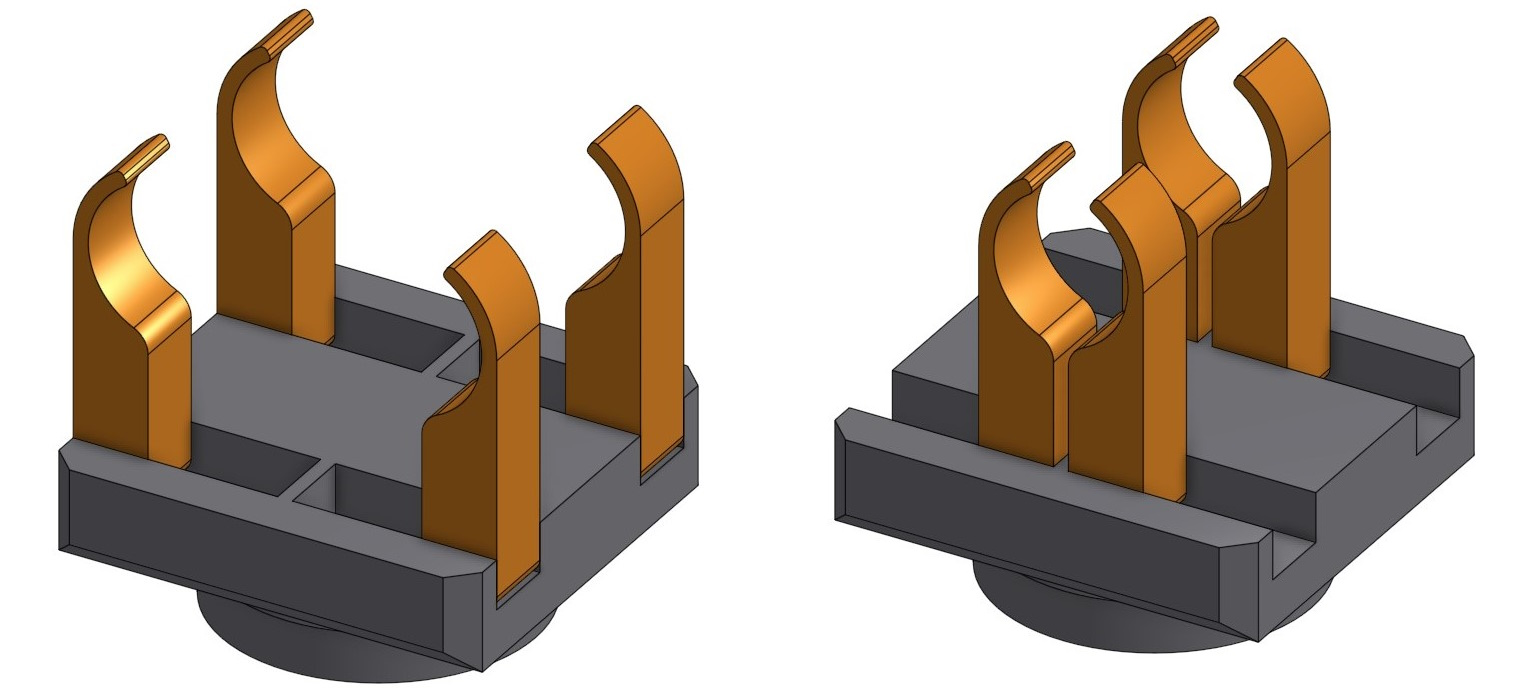
\includegraphics[width=0.75\textwidth]{figures/gripper_dual.jpg}
    \caption{Prihvatnica s četiri prsta; otvorena (lijevo) i zatvorena (desno)}
    \label{fig:gripper-render}
\end{figure}

\begin{figure}[H]
    \centering
    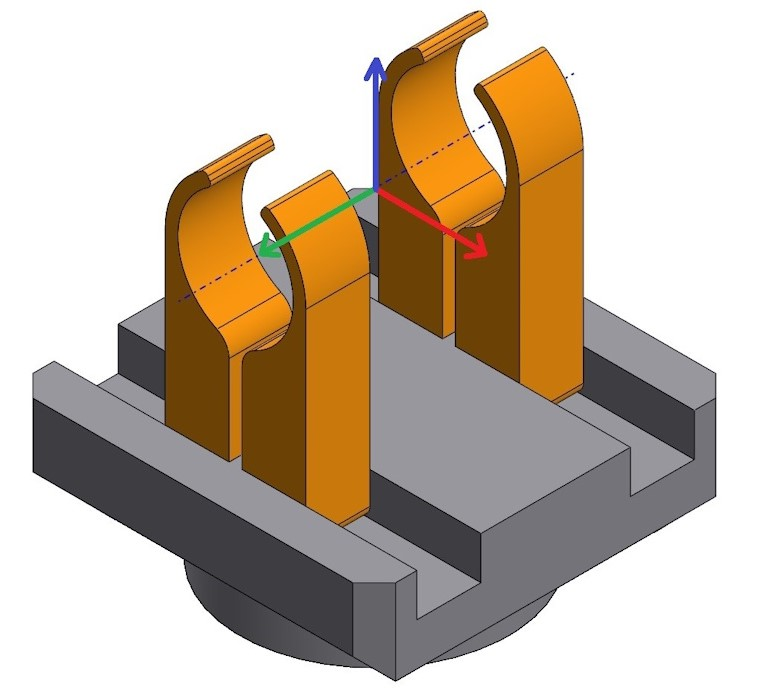
\includegraphics[width=0.45\textwidth]{figures/gripper_tcp.jpg}
    \caption{Položaj vrha alata (\textit{TCP})}
    \label{fig:gripper-tcp}
\end{figure}

\begin{table}[H]
    \centering
    \caption{Značajke prihvatnice}
    \label{tab:gripper}
    \begin{tabular}{@{}ll@{}}
        \toprule
        Značajka                             & Vrijednost          \\
        \midrule
        Promjer prirubnice                   & 63 mm               \\
        Dimenzije nosive ploče               & 85\,$\times$\,85 mm \\
        Duljina prsta                        & 66.5 mm             \\
        Unutarnji polumjer utora             & 16 mm               \\
        Hod po prstu                         & 0--25 mm            \\
        Masa nosivog dijela                  & 442 g               \\
        Masa prsta                           & 30.6 g              \\
        Ukupna masa                          & 564 g               \\
        Položaj vrha alata iznad prirubnice  & 74.85 mm            \\
        Statički koeficijent trenja prstiju  & 1.2                 \\
        Dinamički koeficijent trenja prstiju & 1.0                 \\
        \bottomrule
    \end{tabular}
\end{table}

Vrh alata leži na osi alata, na visini od 74.85 mm iznad prirubnice manipulatora. Ta visina
odgovara središtu unutarnjeg luka kuka pri zatvorenom hvatu, dakle visini na kojoj se nalazi
os uhvaćene šipke. Vrh alata time nije materijalna točka na prihvatnici, nego sjecište osi
alata i osi predmeta u hvatu, čime regulator momente računa oko stvarnog hvatišta.

Prsti su u simulacijskom modelu upravljani pozicijski, s krutošću pogona 20\,000 N/m,
prigušenjem 200 Ns/m i graničnom silom 600 N. Pri vučenju vrata silu prenose djelotvorno samo
dva od četiriju prstiju, jer jedan par radi protiv vlastitog pogona, pa je djelotvorna krutost
hvata polovica nominalne. Ta je pojedinost bitna za tumačenje rezultata u poglavlju
\ref{ch:rezultati}.

\section{Kamera i njezin nosač}
\label{sec:kamera-nosac}

Za detekciju kvake robot je opremljen kamerom Intel RealSense D435, postavljenom na mobilnu
platformu pomoću vlastito izrađenog nosača (slika \ref{fig:camera-mount}).
Sam postupak detekcije i procjene poze opisan je u poglavlju \ref{ch:percepcija};
ovdje je opisana samo montaža i pripadni koordinatni sustavi.

Nosač kamere oblikovan je tako da iskoristi postojeće provrte na platformi. Manipulator se na
platformu pričvršćuje preko četiri provrta promjera 13.3 mm raspoređena po kružnici polumjera
108 mm. Ta je kružnica na platformi izvedena zrcalno s obje strane, a strana suprotna
manipulatoru ostaje slobodna, pa je nosač kamere postavljen upravo na nju. Time montaža ne
zahtijeva nikakvu izmjenu platforme.

\begin{figure}[H]
    \centering
    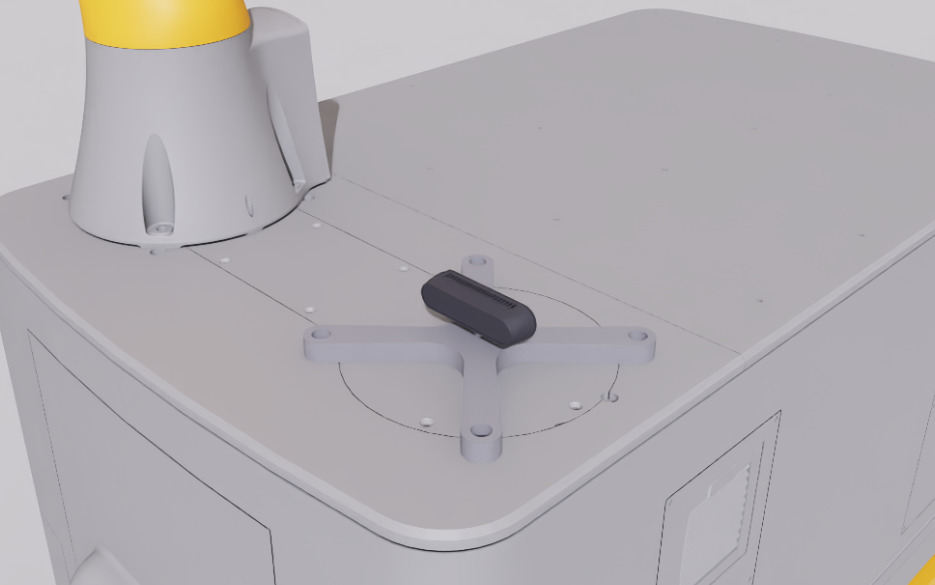
\includegraphics[width=0.7\textwidth]{figures/camera.jpg}
    \caption{Kamera i nosač kamere postavljeni na robotu}
    \label{fig:camera-mount}
\end{figure}

Kamera je smještena na visini gornje plohe platforme, bočno pomaknuta u odnosu na
manipulator. Time je kvaka u vidnom polju i tijekom prilaza i tijekom hvata, a kamera ne
ulazi u radni prostor manipulatora. Nosač je zamišljen kao izradak aditivnom proizvodnjom;
masa od 193 g izračunata je iz obujma modela uz gustoću materijala PETG od
1270 kg/m\textsuperscript{3}.

Kamera u modelu ima dva koordinatna sustava. Prvi je vezan uz kućište i služi za montažu,
a drugi je optički koordinatni sustav u kojem se izražavaju rezultati detekcije. Optički je
zaokrenut u odnosu na kućište prema uobičajenoj konvenciji, pri čemu os $z$ gleda u smjeru
promatranja, a osi $x$ i $y$ leže u ravnini slike. Ta konvencija nije proizvoljna nego je
očekuju biblioteke za obradu slike, pa je zadržana kako procjena poze ne bi zahtijevala
dodatnu pretvorbu.

Kamera podržava i dubinsku sliku, no ona u ovom radu nije korištena. Detekcija vrata i kvake
odvija se isključivo iz slike u boji, pomoću oznaka AprilTag, a postignuta točnost pokazala se
dovoljnom i bez dubinske informacije.

\section{Lidar}
\label{sec:lidar}

Uz kameru, robot je opremljen i dvodimenzijskim laserskim skenerom (lidarom), postavljenim na
prednjoj strani mobilne platforme. Za razliku od kamere, koja služi isključivo detekciji kvake
(poglavlje \ref{ch:percepcija}), lidar se koristi za dvije zadaće vezane uz neposrednu okolinu robota:
otkrivanje prepreka ispred platforme tijekom otvaranja vrata i pronalaženje otvora u zidu radi
prolaska kroz vrata. Obje su zadaće opisane u poglavlju \ref{ch:klasicni}, u opsegu klasičnog
pristupa; pristup temeljen na učenju ne koristi lidar direktno, već očitava pozicije zidova
izravno iz simulatora.

Senzor ima i minimalni domet ispod kojeg mjerenja nisu pouzdana. Budući da je kvaka nakon hvata
na udaljenosti od tek oko 0.65 m od senzora, unutar tog dometa krilo vrata ostaje nevidljivo, pa
je vrijednost minimalnog dometa u konfiguraciji senzora spuštena na 0.05 m.

\section{Modeli vrata}
\label{sec:vrata}

Radnu okolinu čine dva modela vrata, zakretna i klizna (slika \ref{fig:vrata}). Oba su izgrađena od osnovnih
geometrijskih tijela, s istim krilom, a razlikuju se stupnjem slobode gibanja i oblikom
kvake. Zajednička geometrija je namjerna: razlika u ponašanju dvaju pristupa time se ne može
pripisati razlici u dimenzijama ili masi krila.
Geometrijska i inercijska svojstva vrata mogu se vidjeti u tablici \ref{tab:vrata}.

\begin{figure}[H]
    \centering
    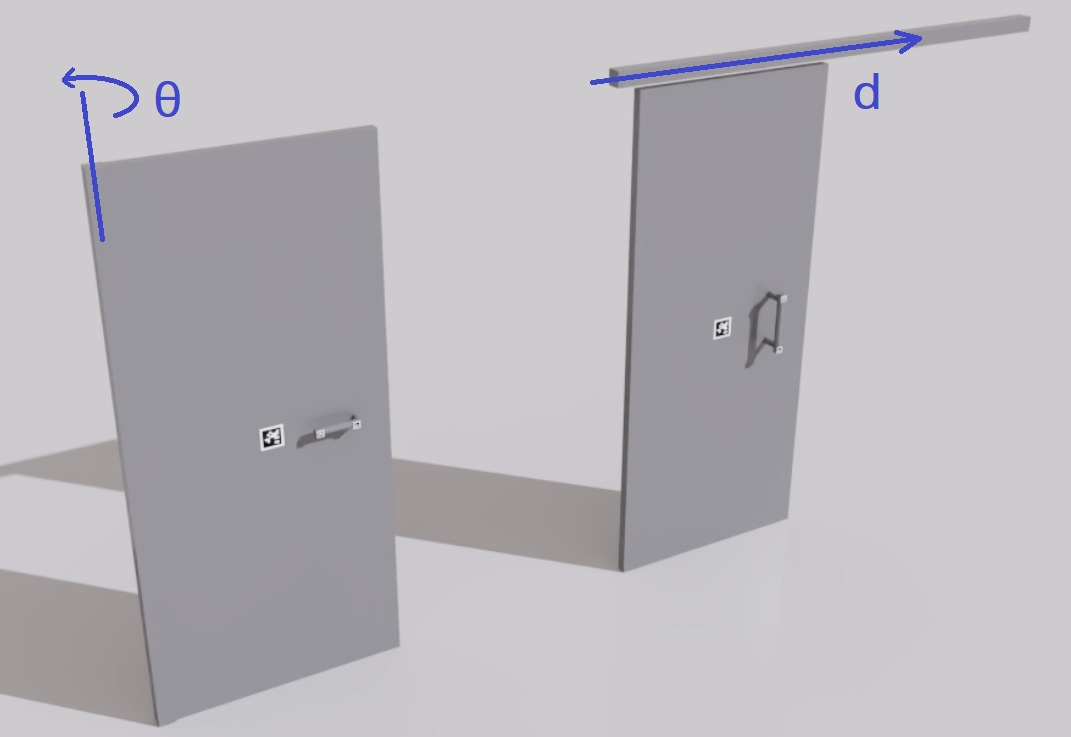
\includegraphics[width=0.9\textwidth]{figures/doors.jpg}
    \caption{Modeli zakretnih i kliznih vrata s označenim stupnjem slobode gibanja}
    \label{fig:vrata}
\end{figure}

\begin{table}[H]
    \centering
    \caption{Geometrija i inercijska svojstva modela vrata}
    \label{tab:vrata}
    \begin{tabular}{@{}lll@{}}
        \toprule
        Veličina             & Zakretna vrata                           & Klizna vrata                                 \\
        \midrule
        Krilo, dimenzije     & 40\,$\times$\,850\,$\times$\,2000 mm     & 40\,$\times$\,850\,$\times$\,2000 mm         \\
        Krilo, masa          & 15 kg                                    & 15 kg                                        \\
        Nepomični dio        & stup 60\,$\times$\,60\,$\times$\,2000 mm & vodilica 60\,$\times$\,2000\,$\times$\,60 mm \\
        Stupanj slobode      & rotacija oko osi $z$                     & translacija duž osi $y$                      \\
        Raspon gibanja       & 0--135 \textdegree{}                     & 0--1.0 m                                     \\
        Kvaka, oblik         & poluga, duljina 160 mm                   & šipka, duljina 250 mm                        \\
        Kvaka, promjer šipke & 28 mm                                    & 28 mm                                        \\
        Kvaka, masa          & 0.35 kg                                  & 0.35 kg                                      \\
        Visina hvatišta      & 1000 mm                                  & 1000 mm                                      \\
        \bottomrule
    \end{tabular}
\end{table}

Kod zakretnih vrata kvaka je izvedena kao poluga usmjerena prema osi šarke, kako je uobičajeno
kod stvarnih vrata. Zglob brave, koji bi omogućio zakretanje kvake, zavaren je u nepomični
zglob u oba pristupa, pa je jedini pokretni stupanj slobode zakretnih vrata os šarke.
Okretanje kvake time je izvan opsega rada; razlog i posljedice te odluke navedeni su u
potpoglavlju \ref{sec:klasicni-limits}. Posljedica koju treba imati na umu jest da se cijeli
moment šarke prenosi trenjem prstiju na šipki kvake.

Kod kliznih vrata kvaka je okomita šipka pričvršćena dvama odstojnicima, pa je hvatište
dostupno s prednje strane krila po cijeloj visini šipke.

Vrata su s obje strane omeđena zidom, izvedenim kao dva zasebna, nepomična elementa,
svaki dimenzija 0.06\,$\times$\,2.5\,$\times$\,2.0 m i mase 15 kg.
Zidovi su postavljeni tako da između njih ostaje slobodan prolaz od 0.85 m,
jednak širini krila vrata, čime nastaje realistična okolina vrata umjesto izoliranog objekta u
praznom prostoru. Ta je okolina preduvjet za dvije zadaće opisane u poglavlju
\ref{ch:klasicni}. Lidar treba stvarnu prepreku da bi u njoj prepoznao otvor, a MoveIt treba
stvarnu geometriju zida da bi je uzeo u obzir pri planiranju gibanja manipulatora.

\subsection{Otpor gibanja i njegova randomizacija}
\label{sec:otpor}

Otpor vrata nije zapisan u geometrijskom modelu, nego se postavlja pri svakom pokretanju
epizode iz zadanog raspona. Time politika nije vezana uz jednu vrijednost otpora, nego uči
raditi na rasponu vrata. Otpor je razdvojen na dva fizikalno različita člana:

\begin{equation}
    \tau_{\mathrm{otpor}} = \tau_{\mathrm{tr}} + d\,\dot{q} ,
    \label{eq:otpor}
\end{equation}

gdje je $q$ koordinata jedinog stupnja slobode vrata, dakle kut zakreta krila kod zakretnih
odnosno pomak krila kod kliznih vrata, a $\dot{q}$ njegova derivacija po vremenu, to jest
brzina otvaranja. Član $\tau_{\mathrm{tr}}$ Coulombovo je trenje, konstantno po iznosu i
neovisno o brzini, dok je $d$ koeficijent viskoznog prigušenja, koji daje otpor razmjeran
brzini. Izraz je zapisan općenito za oba tipa vrata: kod zakretnih su $\tau_{\mathrm{otpor}}$
i $\tau_{\mathrm{tr}}$ momenti, a kod kliznih sile.

Parametri se zadaju u apsolutnim jedinicama, dakle u njutnima za prizmatični i njutnmetrima za
revolutni zglob, a ne kao bezdimenzijski koeficijenti. Da bi se to potvrdilo, provedeno je
mjerenje u simulaciji. Vratima je zadana poznata vrijednost trenja, a zatim je polagano rastućom
silom određena sila pri kojoj se vrata pokrenu. Omjer izmjerene sile pokretanja i zadanog trenja
kretao se između 1.00 i 1.03 za zadane vrijednosti trenja u rasponu od 5 do 60 N, čime
je potvrđeno da zadana vrijednost izravno odgovara sili potrebnoj za pokretanje vrata.

U tablici \ref{tab:randomizacija} mogu se vidjeti rasponi iz kojih su birane vrijednosti otpora vrata:

\begin{table}[H]
    \centering
    \caption{Rasponi randomizacije otpora vrata}
    \label{tab:randomizacija}
    \begin{tabular}{@{}lcc@{}}
        \toprule
        Tip vrata & Trenje    & Prigušenje     \\
        \midrule
        Klizna    & 5--60 N   & 5--50 Ns/m     \\
        Zakretna  & 0.5--5 Nm & 0.5--5 Nms/rad \\
        \bottomrule
    \end{tabular}
\end{table}

Rasponi nisu određeni mjerenjem na stvarnim vratima, nego su usvojeni kao inženjerska
procjena, sa širinom raspona odabranom tako da obuhvati i lagana i teška vrata. Svrha im nije
vjerno preslikati određena vrata, već spriječiti da naučena politika ovisi o jednoj
vrijednosti otpora.

\section{Model robota i pretvorba u simulacijski format}
\label{sec:urdf-usd}

Geometrijski i kinematički model robota opisan je u formatu \textit{Unified Robot Description Format} (URDF). Model manipulatora preuzet
je iz javno dostupnog paketa \texttt{iiwa\_stack} \cite{iiwastack}, a model mobilne platforme
iz proizvođačeve dokumentacije \cite{kuka2024kmriiwa}. Prihvatnica, nosač kamere i oba modela
vrata izrađeni su u sklopu ovog rada. Model je organiziran pomoću \texttt{xacro} predložaka,
tako da se prihvatnica u model uključuje jednim pozivom makronaredbe.

Isaac Sim ne koristi URDF izravno, nego format \textit{Universal Scene Description} (USD). Pretvorba nije jedan korak nego niz
skripti, jer sama pretvorba ne prenosi sve što je za rad potrebno.

Osnovnu pretvorbu obavlja \texttt{convert\_urdf\_usd.py}, proširena inačica alata iz Isaac
Laba. Dvije su postavke pritom bitne:

\begin{itemize}
    \item \textbf{Vrsta kolidera} (engl. \textit{collider type})\textbf{.} Prsti prihvatnice
          moraju se pretvarati postupkom konveksne dekompozicije. Zamotavanje u konveksnu
          ovojnicu zatvorilo bi utore na prstima i prihvatnica ne bi mogla obuhvatiti šipku.
    \item \textbf{Sažimanje nepomičnih zglobova.} Ne smije se primijeniti na model robota, jer
          bi uklonilo zglob na kojem se očitavaju sile i momenti (potpoglavlje \ref{sec:gripper}).
\end{itemize}

Na dobiveni model zatim se primjenjuju tri naknadne skripte:

\begin{itemize}
    \item \texttt{apply\_gripper\_friction.py} pridružuje materijal trenja plohama prstiju i
          kvaka. Pridruživanje se ne može izvesti izravno na složenoj sceni, jer se geometrija
          prsta, referencirana četiri puta iz iste datoteke, pojavljuje kao instancirani sloj u
          koji nije dopušteno upisivati; skripta zato pronalazi stvarni sloj u kojemu se geometrija
          nalazi i materijal upisuje u njega.
    \item \texttt{add\_arm\_ros\_control\_graph.py} umeće graf koji povezuje zglobove
          manipulatora s temama ROS-a 2, čime se model može voditi izvana. Graf mora biti
          ugniježđen unutar stabla osnovnog elementa modela, jer se inače pri referenciranju
          modela u scenu tiho izgubi.
    \item \texttt{add\_camera\_ros\_graph.py} dodaje kameru s izmjerenim unutarnjim parametrima i
          položajem te objavljivanje slike i stabla koordinatnih sustava.
\end{itemize}

Na slici \ref{fig:urdf-usd-pipeline} može se vidjeti dijagram toka pretvorbe datoteka iz URDF formata u
simulatoru koristive datoteke u USD formatu.

\begin{figure}[H]
    \centering
    \begin{tikzpicture}[
            font        = \small,
            box/.style  = {draw, rounded corners=2pt, align=center, inner sep=4pt,
                    minimum height=9mm, minimum width=48mm, fill=black!5},
            data/.style = {box, fill=black!10},
            small/.style= {box, minimum width=44mm, minimum height=8mm},
            note/.style = {font=\scriptsize, align=left, anchor=west, text width=30mm},
            grp/.style  = {draw, dashed, rounded corners=3pt, inner sep=6pt},
            gl/.style   = {font=\scriptsize\itshape, anchor=east},
            ar/.style   = {-{Stealth[length=2mm]}, semithick}
        ]

        % ---------------- robot ----------------
        \node[data]  (rxacro) at (-3.0,0)     {predlošci \texttt{xacro}\\[-1pt]
            \scriptsize robot, prihvatnica, nosač kamere};
        \node[data]  (rurdf)  at (-3.0,-1.9)  {opis robota \texttt{URDF}};
        \node[box]   (rconv)  at (-3.0,-3.8)  {\texttt{convert\_urdf\_usd.py}};
        \node[data]  (rusd0)  at (-3.0,-5.7)  {osnovni model robota \texttt{USD}};

        \node[small] (fric) at (-3.0,-7.7)  {\texttt{apply\_gripper\_friction.py}};
        \node[small] (rosg) at (-3.0,-9.1)  {\texttt{add\_arm\_ros\_control\_graph.py}};
        \node[small] (camg) at (-3.0,-10.5) {\texttt{add\_camera\_ros\_graph.py}};
        \node[grp, fit=(fric)(rosg)(camg)] (gpost) {};
        \node[gl] at (gpost.west) {naknadna obrada};

        \node[data] (rusd1) at (-3.0,-12.6) {potpuni model robota \texttt{USD}};

        % ---------------- vrata ----------------
        \node[data, minimum width=44mm] (durdf) at (4.6,-5.7)
        {opis vrata \texttt{URDF}\\[-1pt]\scriptsize zakretna i klizna};
        \node[box,  minimum width=44mm] (dconv) at (4.6,-7.6)
        {\texttt{convert\_urdf\_usd.py}};
        \node[data, minimum width=44mm] (dusd)  at (4.6,-9.6)
        {modeli vrata \texttt{USD}\\[-1pt]\scriptsize inačice s oznakama i bez njih};

        % ---------------- izlazi ----------------
        \node[box, minimum width=42mm] (basej) at (-6.2,-14.8)
        {\texttt{add\_base\_joints.py}\\[-1pt]\scriptsize tri pomoćna zgloba platforme};
        \node[data, minimum width=42mm] (rlasset) at (-6.2,-16.9)
        {model za učenje\\[-1pt]\scriptsize \texttt{kmr\_iiwa\_full\_rl.usd}};

        \node[box, minimum width=52mm] (bis) at (0.9,-14.8)
        {\texttt{build\_integration\_scene.py}\\[-1pt]\scriptsize dodavanje podloge scene};
        \node[data, minimum width=52mm] (scene) at (0.9,-16.9)
        {integracijska scena\\[-1pt]\scriptsize \texttt{integration\_test\_*.usd}};

        % ---------------- tok ----------------
        \draw[ar] (rxacro) -- (rurdf);
        \draw[ar] (rurdf)  -- (rconv);
        \draw[ar] (rconv)  -- (rusd0);
        \draw[ar] (rusd0)  -- (gpost.north -| rusd0.south);
        \draw[ar] (fric)   -- (rosg);
        \draw[ar] (rosg)   -- (camg);
        \draw[ar] (gpost.south -| rusd1.north) -- (rusd1);

        \draw[ar] (durdf) -- (dconv);
        \draw[ar] (dconv) -- (dusd);

        \draw[ar] (rusd1.south) -- ++(0,-0.9) -| (basej.north);
        \draw[ar] (rusd1.south) -- ++(0,-0.9) -| (bis.north);
        \draw[ar] (basej) -- (rlasset);
        \draw[ar] (bis)   -- (scene);
        \draw[ar] (dusd.south) -- (4.6,-14.8) -- (bis.east);

        % ---------------- napomene ----------------
        \node[note] at (-0.4,-2.85) {sažimanje makronaredbi};
        \node[note] at (-0.4,-4.75) {konveksna dekompozicija kolidera;
            bez sažimanja nepomičnih zglobova};

    \end{tikzpicture}
    \caption{Postupak izrade simulacijskog modela iz opisa robota i vrata}
    \label{fig:urdf-usd-pipeline}
\end{figure}

Za učenje se koristi zasebna inačica modela. Iz modela vrata uklonjeni su nosivi elementi
oznaka za percepciju, jer tijela mase 0.001 kg uz krilo mase 15 kg loše uvjetuju numerički
postupak rješavanja. Nazivi članaka i zglobova ujednačeni su između obaju tipova vrata, čime
jedna programska implementacija okruženja poslužuje oba tipa bez grananja po tipu vrata.

\subsection{Gibanje mobilne platforme}
\label{sec:baza-model}

Mecanum kotači nisu simulirani kao tijela u kontaktu s podlogom. Umjesto toga, gibanje
platforme zadaje se kinematički: naredba brzine iz poruke \texttt{/cmd\_vel} pretvara se u
pomake platforme po osima $x$ i $y$ te zakret oko osi $z$. U okruženju za učenje isti je
mehanizam ostvaren trima pomoćnim zglobovima umetnutima između nepomičnog ishodišta i članka
platforme, pa se platforma giba kao dio iste kinematičke strukture kao i manipulator.

Korijen kinematičke strukture pritom ostaje nepomičan. To je nužno jer regulator u
operacijskom prostoru, opisan u poglavlju \ref{ch:rl}, računa jakobijan i matricu inercije uz
pretpostavku nepomičnog korijena; uz slobodan korijen kompenzacija gravitacije ispada
neispravna.

Zanemarivanje dinamike kotača pojednostavljenje je koje uklanja proklizavanje, elastičnost
valjaka i ograničenja pogona kotača. Za zadatak u kojem se platforma giba malim brzinama i u
kojem su zanimljive sile na vrhu alata, a ne na kotačima, to je prihvatljivo, ali ograničava
prenosivost rezultata na stvarnog robota. Ograničenje je navedeno u poglavlju
\ref{ch:zakljucak}.

\section{Simulacijsko okruženje}
\label{sec:isaac}

Simulacija se izvodi u okruženju NVIDIA Isaac Sim, uz biblioteku Isaac Lab
\cite{isaaclab} za paralelno učenje. Fizika se rješava pogonom PhysX. Cijeli je rad proveden u
simulaciji jer stvarni robot nije bio dostupan, a zadatak zahtijeva velik broj ponavljanja
interakcije s kontaktom, što na stvarnom robotu nije izvedivo u opsegu završnog rada.

Bitna je značajka postava razdvajanje odgovornosti: geometrijski model nosi topologiju i
geometriju, a sva pojačanja pogona i svojstva otpora zadaju se u konfiguraciji okruženja. Time
se izbjegava da se naučena politika veže uz jednu konkretnu datoteku modela umjesto uz raspon
uvjeta.

Pogoni osi manipulatora postavljeni su na nultu krutost i prigušenje. Momente računa regulator
u operacijskom prostoru i zadaje ih izravno; da je zadržana krutost iz pretvorbe, pogon i
regulator djelovali bi jedan protiv drugoga i krutost koju politika zada ne bi imala učinka.
Pogon platforme brzinski je, s prigušenjem $10^4$, a pogon prstiju pozicijski, s vrijednostima
navedenima u potpoglavlju \ref{sec:gripper}.

Programska i sklopovska konfiguracija može se vidjeti u tablici \ref{tab:okruzenje}.

\begin{table}[H]
    \centering
    \caption{Programska i sklopovska konfiguracija}
    \label{tab:okruzenje}
    \begin{tabular}{@{}ll@{}}
        \toprule
        Stavka                      & Vrijednost                         \\
        \midrule
        Operacijski sustav          & Ubuntu 22.04 LTS                   \\
        Simulator                   & NVIDIA Isaac Sim 5.1.0             \\
        Biblioteka za učenje        & Isaac Lab 2.3.2                    \\
        Robotski operacijski sustav & ROS 2 Humble                       \\
        Python (Isaac Lab)          & 3.11.15                            \\
        Python (ROS 2)              & 3.10.12                            \\
        \midrule
        Procesor                    & AMD Ryzen 7 260                    \\
        Grafička kartica            & NVIDIA GeForce RTX 5050, 8 GB VRAM \\
        Radna memorija              & 32 GB DDR5                         \\
        \bottomrule
    \end{tabular}
\end{table}

\section{Programska arhitektura}
\label{sec:ros2}

Softver je podijeljen u pakete unutar radnog prostora ROS 2, navedene u tablici
\ref{tab:paketi}. Podjela slijedi funkcionalne cjeline rada: opis robota, percepcija, veza sa
simulatorom, izvođenje zadatka, konfiguracija i pokretanje sustava.

\begin{table}[H]
    \centering
    \caption{Paketi radnog prostora ROS 2}
    \label{tab:paketi}
    \begin{tabular}{@{}ll@{}}
        \toprule
        Paket                              & Sadržaj                                                \\
        \midrule
        \texttt{kmr\_iiwa\_description}    & modeli robota, prihvatnice, kamere i vrata             \\
        \texttt{kmr\_iiwa\_perception}     & detekcija oznaka, fuzija poze, procjena sile i momenta \\
        \texttt{kmr\_iiwa\_sim\_bridge}    & veza sa simulatorom: platforma, prihvatnica, kamera    \\
        \texttt{kmr\_iiwa\_task}           & izvođenje zadatka i procjena ograničenja gibanja       \\
        \texttt{kmr\_iiwa\_moveit\_config} & konfiguracija planiranja gibanja manipulatora          \\
        \texttt{kmr\_iiwa\_bringup}        & pokretanje cjelokupnog sustava                         \\
        \bottomrule
    \end{tabular}
\end{table}

Isaac Sim nema izvornu podršku za sučelje \texttt{ros2\_control}, pa je veza sa simulatorom
ostvarena vlastito izrađenim čvorovima koji prevode poruke ROS 2 u naredbe simulatoru. Upravljanje
prihvatnicom namjerno je izvedeno kao potpuno odvojena cjelina: jedini čvor koji zna da
prihvatnica ima četiri prizmatična zgloba i hod od 25 mm jest njezin upravljački čvor, dok
ostatak sustava prihvatnicu vidi kroz jedan broj u rasponu od nula do jedan, uz povratnu
informaciju o trenutnom položaju i o tome je li zaustavljena prije dolaska u zadani položaj.
Time je zadovoljen zahtjev iz potpoglavlja \ref{sec:gripper} da se prihvatnica može zamijeniti
bez izmjena u ostatku sustava.

Na slici \ref{fig:arch-klasicni} može se vidjeti dijagram arhitekture za klasično učenje.

\begin{figure}[H]
    \centering
    \begin{tikzpicture}[
            font       = \small,
            box/.style = {draw, rounded corners=2pt, align=center, inner sep=4pt,
                    minimum height=9mm, fill=black!5},
            grp/.style = {draw, dashed, rounded corners=3pt, inner sep=7pt},
            gl/.style  = {font=\scriptsize\itshape, anchor=east},
            tl/.style  = {font=\scriptsize\ttfamily, fill=white, inner sep=1.5pt},
            ar/.style  = {-{Stealth[length=2mm]}, semithick}
        ]

        % --- simulator ---
        \node[box, minimum width=112mm, fill=black!10] (sim) at (0,0)
        {Isaac Sim --- scena: robot, vrata, fizika kontakta};

        % --- percepcija ---
        \node[box, minimum width=44mm] (tag) at (-2.6,-2.7)
        {detekcija oznaka\\i fuzija poze};
        \node[box, minimum width=40mm] (wr)  at ( 2.8,-2.7)
        {procjena sile\\i momenta};
        \node[grp, fit=(tag)(wr)] (gperc) {};
        \node[gl] at (gperc.west) {\texttt{kmr\_iiwa\_perception}};

        % --- zadatak ---
        \node[box, minimum width=50mm] (task) at (-2.2,-5.8)
        {izvođenje zadatka\\[-1pt]\scriptsize prilaz, hvat, procjena, otvaranje};
        \node[box, minimum width=30mm] (moveit) at (3.6,-5.8) {MoveIt 2\\planiranje};
        \node[grp, fit=(task)] (gtask) {};
        \node[gl] at (gtask.west) {\texttt{kmr\_iiwa\_task}};

        % --- most prema simulatoru ---
        \node[box, minimum width=26mm] (cmdvel) at (-3.6,-8.8) {platforma};
        \node[box, minimum width=26mm] (grip)   at ( 0.0,-8.8) {prihvatnica};
        \node[box, minimum width=26mm] (armg)   at ( 3.6,-8.8) {manipulator};
        \node[grp, fit=(cmdvel)(grip)(armg)] (gbridge) {};
        \node[gl] at (gbridge.west) {\texttt{kmr\_iiwa\_sim\_bridge}};

        % --- simulator -> percepcija ---
        \draw[ar] (sim.south -| tag.north) -- (tag.north);
        \draw[ar] (sim.south -| wr.north)  -- (wr.north);
        \node[tl] at (-2.6,-1.35) {/camera/color/image\_raw};
        \node[tl] at ( 2.8,-1.35) {/joint\_states};

        % --- simulator -> zadatak (lidar, izravno, bez zasebnog obradnog čvora) ---
        \draw[ar] (sim.south -| 5.2,0) -- (5.2,-4.6) -- (1.2,-4.6) -- (1.2,-5.8) -- (task.east);
        \node[tl] at (3.2,-4.6) {/scan};

        % --- percepcija -> zadatak ---
        \draw[ar] (tag.south) -- (tag.south |- gtask.north);
        \draw[ar] (wr.south) -- ++(0,-1.1) -| ($(task.north)+(1.6,0)$);
        \node[tl] at (-2.6,-4.25) {/perception/handle\_pose};
        \node[tl] at ( 2.8,-4.25) {/estimation/tcp\_wrench};

        % --- zadatak <-> MoveIt ---
        \draw[{Stealth[length=2mm]}-{Stealth[length=2mm]}, semithick]
        (moveit.west) -- (task.east);

        % --- zadatak -> most ---
        \draw[ar] ($(task.south)+(-1.4,0)$) -- ++(0,-1.1) -| (cmdvel.north);
        \draw[ar] ($(task.south)+(1.4,0)$)  -- ++(0,-1.7) -| (grip.north);
        \draw[ar] (moveit.south) -- (armg.north);
        \node[tl] at (-3.6,-7.35) {/cmd\_vel};
        \node[tl] at ( 0.0,-7.35) {/gripper\_cmd};
        \node[tl] at ( 3.6,-7.35) {trajektorija};

        % --- most -> simulator (zatvaranje petlje desno) ---
        \draw[ar] (gbridge.east) -- ++(1.3,0) |- (sim.east);
        \node[tl, rotate=90] at (6.3,-4.4) {naredbe simulatoru};

    \end{tikzpicture}
    \caption{Programska arhitektura klasičnog pristupa}
    \label{fig:arch-klasicni}
\end{figure}

Pristup temeljen na učenju koristi bitno jednostavniju arhitekturu (slika \ref{fig:arch-rl}). Tijekom učenja ROS 2 nije
u regulacijskoj petlji: okruženje, regulator i politika izvode se unutar Isaac Laba, izravno
nad tenzorima na grafičkoj kartici. Razlog je paralelizacija --- učenje se izvodi u više
stotina istovremenih okruženja, a posredovanje kroz ROS 2 bilo bi usko grlo. Veza s ROS-om
potrebna je tek pri izvođenju naučene politike izvan simulacije, što nije bilo u opsegu ovog
rada i opisano je u poglavlju \ref{ch:rezultati}.

\begin{figure}[H]
    \centering
    \begin{tikzpicture}[
            font       = \small,
            box/.style = {draw, rounded corners=2pt, align=center, inner sep=4pt,
                    minimum height=9mm, minimum width=32mm, fill=black!5},
            grp/.style = {draw, dashed, rounded corners=3pt, inner sep=7pt},
            gl/.style  = {font=\scriptsize\itshape, anchor=east},
            tl/.style  = {font=\scriptsize, fill=white, inner sep=1.5pt},
            ar/.style  = {-{Stealth[length=2mm]}, semithick}
        ]

        \node[box, minimum width=104mm, fill=black!10] (phys) at (0,0)
        {PhysX --- $N$ paralelnih okruženja na grafičkoj kartici};

        \node[box] (obs) at (-3.4,-2.7) {opažanje};
        \node[box] (pol) at ( 0.0,-2.7) {politika\\[-1pt]\scriptsize neuronska mreža};
        \node[box] (act) at ( 3.4,-2.7) {akcija};
        \node[grp, fit=(obs)(pol)(act)] (gpol) {};
        \node[gl] at (gpol.west) {upravljačka petlja};

        \node[box, minimum width=54mm] (osc) at (1.0,-5.4)
        {regulator u operacijskom prostoru\\[-1pt]\scriptsize varijabilna impedancija};

        \node[box] (ppo) at (-2.6,-7.9) {PPO\\[-1pt]\scriptsize \texttt{rsl\_rl}};
        \node[box] (rew) at ( 3.0,-7.9) {nagrada};
        \node[grp, fit=(ppo)(rew)] (glearn) {};
        \node[gl] at (glearn.west) {učenje};

        % --- upravljačka petlja ---
        \draw[ar] (phys.south -| obs.north) -- (obs.north) node[tl, midway] {stanje};
        \draw[ar] (obs.east) -- (pol.west);
        \draw[ar] (pol.east) -- (act.west);
        \draw[ar] (act.south) -- (act.south |- osc.north)
        node[tl, midway] {pomak i krutost};

        % momenti: desnom stranom natrag u fiziku
        \draw[ar] (osc.east) -- (6.0,-5.4) -- (6.0,-0.225) -- (phys.east);
        \node[tl, rotate=90] at (6.0,-3.0) {momenti};

        % --- petlja učenja ---
        \draw[ar] (phys.east) ++(0,0.15) -- (7.4,0.15) -- (7.4,-7.9) -- (rew.east);
        \node[tl, rotate=90] at (7.4,-4.4) {napredak, sila};
        \draw[ar] (rew.west) -- (ppo.east);

        % ažuriranje: lijevom stranom, iznad regulatora
        \draw[ar] (ppo.north) -- (-2.6,-4.35) -- (0,-4.35) -- (pol.south);
        \node[tl] at (-1.3,-4.35) {ažuriranje težina};

    \end{tikzpicture}
    \caption{Programska arhitektura pristupa temeljenog na učenju}
    \label{fig:arch-rl}
\end{figure}